\chapter{Effect of the long correlated disorder in the light emission statistics of a two dimensional dipole lattice\label{chap6}}

\section{Introduction}

The study of the Purcell effect (see chapter (\ref{chap2:Dipole_radiation})) in idealised systems has attracted attention in recent years, mainly due to the possibility of create such systems. This last fact has stimulated the interest of wave propagation through disordered media \cite{wiersma2013disordered}.
%In chapter (\ref{chap2:Dipole_radiation}) we introduce the Purcell effect, a phenomenon where the lifetime of an excited atomic state depends of the environment that is embedded. In recent years, with the possibility of creating nanostructured materials, there has been an increase of the interest in wave propagation through disordered media \cite{wiersma2013disordered}. 
Examples like enhanced backscattering \cite{Ishimaru_1985,Mark_1998},
photon localization \cite{wiersma1997localization} random lasing \cite{Lawandy_1994,Cao_2000}, or photonic membranes \cite{Caze_2013, garcia2012nonuniversal} can be found in the literature. Also, the behaviour of light coupled to disordered matter has been analysed from the point of view of diluted cold atom systems where atoms are scarcely located in an optical lattice \cite{bloch2008many, sherson2010single, bloch2012quantum, froufe2009threshold}.
In complex systems like liquids, colloids, granular or biological
materials, the dynamic modification of the environment or the movement
of the emitter implies the need for a statistical study of the decay rate \cite{Froufe_PRA_2007,Froufe_2008,Sapienza_2011}. In these random systems, the decay rate exhibits a non-Gaussian, long-tailed distribution, where large enhancements of the Purcell factor are attributed to strong fluctuations in the local density of states induced by the near-field scattering
\cite{Martorell_1991,krachmalnicoff2010fluctuations,Sapienza_2011}.
These rare events create optical modes confined in a small volume around the source.\\
In most cases, previously studied disorder was produced in a random
way, that is, scatterers were distributed throughout the lattice randomly.
Real systems, however, can be realised with other kinds of disorder,
where the locations of particles are correlated. In particular,
structural disorder with long-range correlation (LRC) has been found
for instance in x-ray and neutron critical scattering experiments
in systems undergoing magnetic and structural phase transition \cite{ShiraneI,ShiraneII,ShiraneIII,ShiraneIV}.
This correlation effect in magnetic systems may be modelled by assuming
a spatial distribution of critical temperatures with a correlation function obeying a slow power law decay \cite{Weinrib,Altarelli,BallesterosIV}.
Spatial correlations in disordered scattering materials have been shown to dramatically modify the light transport properties, in particular, light scattering mean-free-path presents strong chromatic dispersion \cite{Rojas_2004, Froufe_2009,caze2010near,Caze_2013}.

In this chapter, we explore the dependence of the decay rate of an emitter in a two-dimensional system as a function of the particle's correlations.
Long-range correlated distributions of scatterers are produced by using a thermal order-disorder distribution governed by a characteristic ordering temperature ($\theta$) \cite{Marques,MarquesII}. In particular, the quenched randomness is implemented using a lattice-gas model equivalent to a thermally-diluted ferromagnetic two dimensional (2D) Ising lattice at a temperature $(\theta)$. We perform extensive calculations of the fluorescence decay rate of a point emitter embedded in a system of nanoparticles  statistically distributed according to a 2D lattice-gas model near the critical point. As we will show, for short-range correlations (high-temperature thermalisation), the Purcell factors present a non-Gaussian long-tailed statistic where events with large Purcell factors are extremely rare. Interestingly, as we approach the critical point where  the  spatial correlation range diverges, the statistics evolves towards a bimodal distribution with a well-defined peak at high enhancement factors, while other peak remains at values corresponding to free space. Our numerical results strongly resemble those obtained experimentally in resonant thin metallic films near percolation \cite{krachmalnicoff2010fluctuations}, which suggest  long-range correlations as a possible origin of the large fluctuations of experimental decay rates in disordered metal films. \\
In Sec. (\ref{chap:chap6_statement}) we describe the physical system and introduce the model under consideration. Sec. (\ref{chap:chap6_discussion}) is devoted to the presentation of the numerical results and discussion. In Sec. (\ref{chap:chap6_conclusions}) we present the central conclusions of this work.

\section{Statement of the model \label{chap:chap6_statement}}

Let us consider the lattice system sketched in Fig. (\ref{fig:crystalline_structure}). The nodes of this square lattice are taken as the possible location points of the optical dipoles by taking into account the following mechanism: After thermalisation of the pure Ising model at temperature $\theta$, the spins with $s=1$ are taken as the locations of the scattering dipoles, while spins with $s=-1$ are considered as dipole vacancies (\textit{i.e.}, sites with no optical response). The structure of the realisation so constructed is fixed thereafter for all subsequent optical-decay-rate studies.\\

\begin{figure}[h]
\begin{centering}
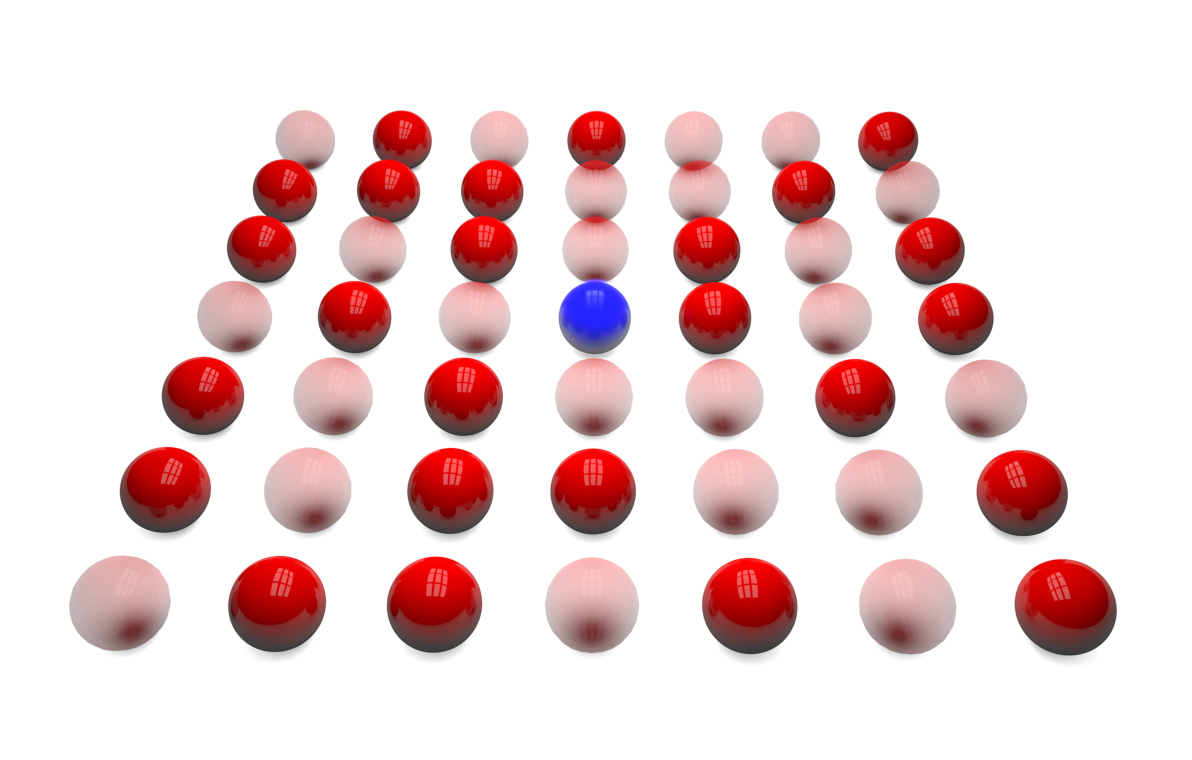
\includegraphics[width=10cm]{chapter_6/figures/fig_1} 
\par\end{centering}
\caption{Schematic representation of a crystalline structure with an edge ($D$)
of 7 particles. The transparent spheres represent the removed particles. The dipole emitter is represented by the blue sphere
and the scatterers by red spheres.\label{fig:crystalline_structure}}
\end{figure}

The structures are generated from the following idea:\\
We start by consider a square lattice with $D \times D$ sites, each site with a set of four adjacent sites. For each lattice site with coordinates $i,j$, there is a discrete variable $\sigma_{i,j}$ such that $\sigma_{i,j} \in \left\{-1,1\right\}$, representing the site spin. So, a system configuration, in this context, is an assignment of a spin value to each lattice site. For any two adjacent sites, $\sigma_{i,j}$ and $\sigma_{\left(i+\zeta\right),\left(j+\zeta\right)}$ with $\zeta = \left\{-1,1\right\}$, there is an interaction $J_{\left[{i,j}\right]\left[{\left(i+\zeta\right),\left(j+\zeta\right)}\right]}$ that allow us to calculate the energy associated to the spin, given by the Hamiltonian:

\begin{equation}
H\left(\sigma_{i,j}\right) = -J_{\left[i,j\right]\left[i,j+1\right]}\sigma_{i,j}\sigma_{i,j+1} - J_{\left[i,j\right]\left[i,j-1\right]}\sigma_{i,j}\sigma_{i,j-1} - \atop -J_{\left[i,j\right]\left[i+1,j\right]}\sigma_{i,j}\sigma_{i+1,j} -J_{\left[i,j\right]\left[i-1,j\right]}\sigma_{i,j}\sigma_{i-1,j}.
\end{equation}
Initially, we generate a random structure, a square lattice where a random spin is assigned for each site. We assume that the interaction between spins is $J_{\left[{i,j}\right]\left[{\left(i+\zeta\right),\left(j+\zeta\right)}\right]}=1$. \\
For each site, we calculate the difference between energies when the spin $\sigma_{i,j}$ assumes the value of $1$ and $-1$, $\delta E = H\left(-\sigma_{i,j}\right)-H\left(\sigma_{i,j}\right)$. 
So, considering the Metropolis algorithm, the system changes its configuration (from $\sigma_{i,j}$ to $-\sigma_{i,j}$) with a probability $p = e^{-\delta E/\theta}$, with $\theta$ the temperature of the system. \\
If $\delta E < 0$, the probability is $p = 1$ and the new spin configuration is accepted. If $\delta E > 0$ the probability of acceptance the new spin is smaller than $1$. We generate a random number between the interval $\left[0,1\right]$ and we compare with $p$. If the random number is larger than $p$, the new spin configuration is refused, otherwise is accepted.\\
This process is repeated to all spin positions a large number of times to obtain independent configurations, \textit{i.e.}, that two consecutive configurations be uncorrelated. For the optical calculation, we only consider configurations where the amount of spins $1$ is between $45\%$ and $55\%$. In this work, for each temperature and lattice dimensions, we generate $10^6$ different configurations to perform optical calculations. As already said, the spins with $s=1$ are taken as the locations of the scattering dipoles, while spins with $s = -1$ are considered as dipole vacancies.
%In order to be able to compare both cases we only consider systems with a concentration in the range between $c=0.45$ and $c=0.55$.
The construction of these thermally disordered systems has been largely explored by Marqu�s \textit{et al.} \cite{Marques,MarquesII}.

In these systems, the correlation function between point dipoles separated by a distance $r$  is  given by the spin-spin correlation function \cite{Yeomans}:

\begin{equation}
g(r)\sim r^{-\tau}exp^{-r/\xi}
\end{equation}
with $\xi$ being the correlation length and $\tau$ a characteristic number depending on the system. The correlation length, near the critical temperature of the Ising model ($T_ {c}$), depends on the ordering temperature with a power law given by $\xi\sim(\theta-T_{c})^{-\nu}$, where $\nu=1$ and $T_{c}=2/ln(1+\sqrt{2})$ for the two-dimensional Ising system.\\
Hence, if a high ordering temperature ($\theta\gg T_{c}$) is used to generate a particular realisation, the correlation function of the equilibrium thermal disposition of the dipoles is going to be given by $g(r)\sim exp(-r/\xi)$, {\it i.e.}, we have a random (short-range correlated) disorder similar to the one used in previous investigations \cite{Froufe_2008, Martorell_1991,Sapienza_2011}. However, if $\theta$ happens to coincide with the characteristic critical temperature of the pure Ising model ($\theta=T_{c}$) then $\xi \rightarrow \infty$ and we are going to have scatterers randomly located, but following a long-range correlated distribution given by $g(r) \sim r^{-\tau}$.  The dispersion on dipole concentration ($c$) obtained by a thermal distribution at $\theta=T_{c}$ is larger than the one obtained when scatterers are randomly distributed with no correlation.

We consider a square lattice with lateral size $D$, where the emitter is placed in the central position of the lattice and oriented out of plane (see Fig. (\ref{fig:crystalline_structure})). 

We consider a particular frequency ($\omega = \omega_{0}$) and an associated particular wavenumber ($k =\omega_{0}/c$) at which dipoles are in resonance with the electromagnetic radiation, meaning that the polarisability is now given by $\alpha = i6\pi/k^3$, like discussed in chapter (\ref{sec:chap2_resonant}). 
In the presence of $\mathcal{N}$ dipole scatterers, the electric field at some point $\mathbf{r}$ is obtained by the superposition principle:

\begin{equation}
{\mathbf{E}\left(\mathbf{r}\right)=\frac{k^{2}}{\epsilon_{0}}\mathbf{G}\left(\mathbf{r},\mathbf{r}_{0}\right)\boldsymbol{\mu}+\atop +\frac{k^{2}}{\epsilon_{0}}\sum_{{m=1}}^{N}{\mathbf{G}\left(\mathbf{r},\mathbf{r}_{m}\right)}\mathbf{p}_{m},}\label{eq:electric_field}
\end{equation}
where $\mathbf{r}_{0}$ is the position of the dipole emitter $\boldsymbol{\mu}$, $\mathbf{r}_{m}$ is the position of scatterer $m$ and $\mathbf{p}_{m}=\epsilon_{0}\alpha\mathbf{E}(\mathbf{r}_{m})$ is the value of the induced dipole located at $\mathbf{r}_{m}$. To obtain the value of all induced dipoles we should solve the electric fields in Eq. (\ref{eq:electric_field}) by considering the coupled dipole method (see chapter (\ref{chap:chap2_DDA})).
The second term on the right-hand side of Eq. (\ref{eq:electric_field})
represents the modification of the free-space dyadic Green function
due to the presence of the scatterers. The scattered field in the dipole emitter position is then given by:

\begin{equation}
\mathbf{E}_{s}\left(\mathbf{r}_{0}\right)=k^{2}\alpha\sum_{{m=1}}^{N}{\mathbf{G}\left(\mathbf{r}_{0},\mathbf{r}_{m}\right)}\mathbf{E}(\mathbf{r}_{m}).\label{eq:scattering_field}
\end{equation}
Once the scattered field is known, the normalized spontaneous decay rate
$\Gamma$ of a dipole $\boldsymbol{\mu}$, in the weak-coupling regime, is given by:

\begin{equation}
\frac{\Gamma}{\Gamma_{0}}=1+\frac{6\pi\epsilon_{0}}{\left|\boldsymbol{\mu}\right|^{2}k^{3}}\Im[\boldsymbol{\mu}^*\cdot\mathbf{E}_{s}\left(\mathbf{r}_{0}\right)],\label{decay_rate}
\end{equation}
where $\Im$ is the imaginary part and $\Gamma_{0}$ is the decay rate of the emitter in free space. It is important to take into account that the expression for the spontaneous decay rate we are considering is an approximation valid only for the weak interacting field. In fact, Eq. (\ref{decay_rate}) is obtained by quantum electrodynamics calculations of the spontaneous decay rate of an atomic system in an inhomogenous medium when the weak-coupling regime approximation is considered \cite{Novotny_PNO_2012}.

\section{Results and discussion \label{chap:chap6_discussion}}

First, we analyse the full crystalline configuration and calculate the normalized decay rate of the emitter, positioned in the center of the structure, as a function of the ratio between the lattice parameter $a$ and the resonance wavelength considered $\lambda=\frac{2\pi}{k}$. We fix the wavelength of the emitter and we vary the lattice parameter.\\
Results presented in Fig. (\ref{fig:crystalline_spectrum}) for a system with lateral dimension $D=23$, allow us to identify a maximum at $\frac{a}{\lambda}=0.44$ with value $\Gamma/\Gamma_{0}\sim7$. 

\begin{figure}[h]
\begin{centering}
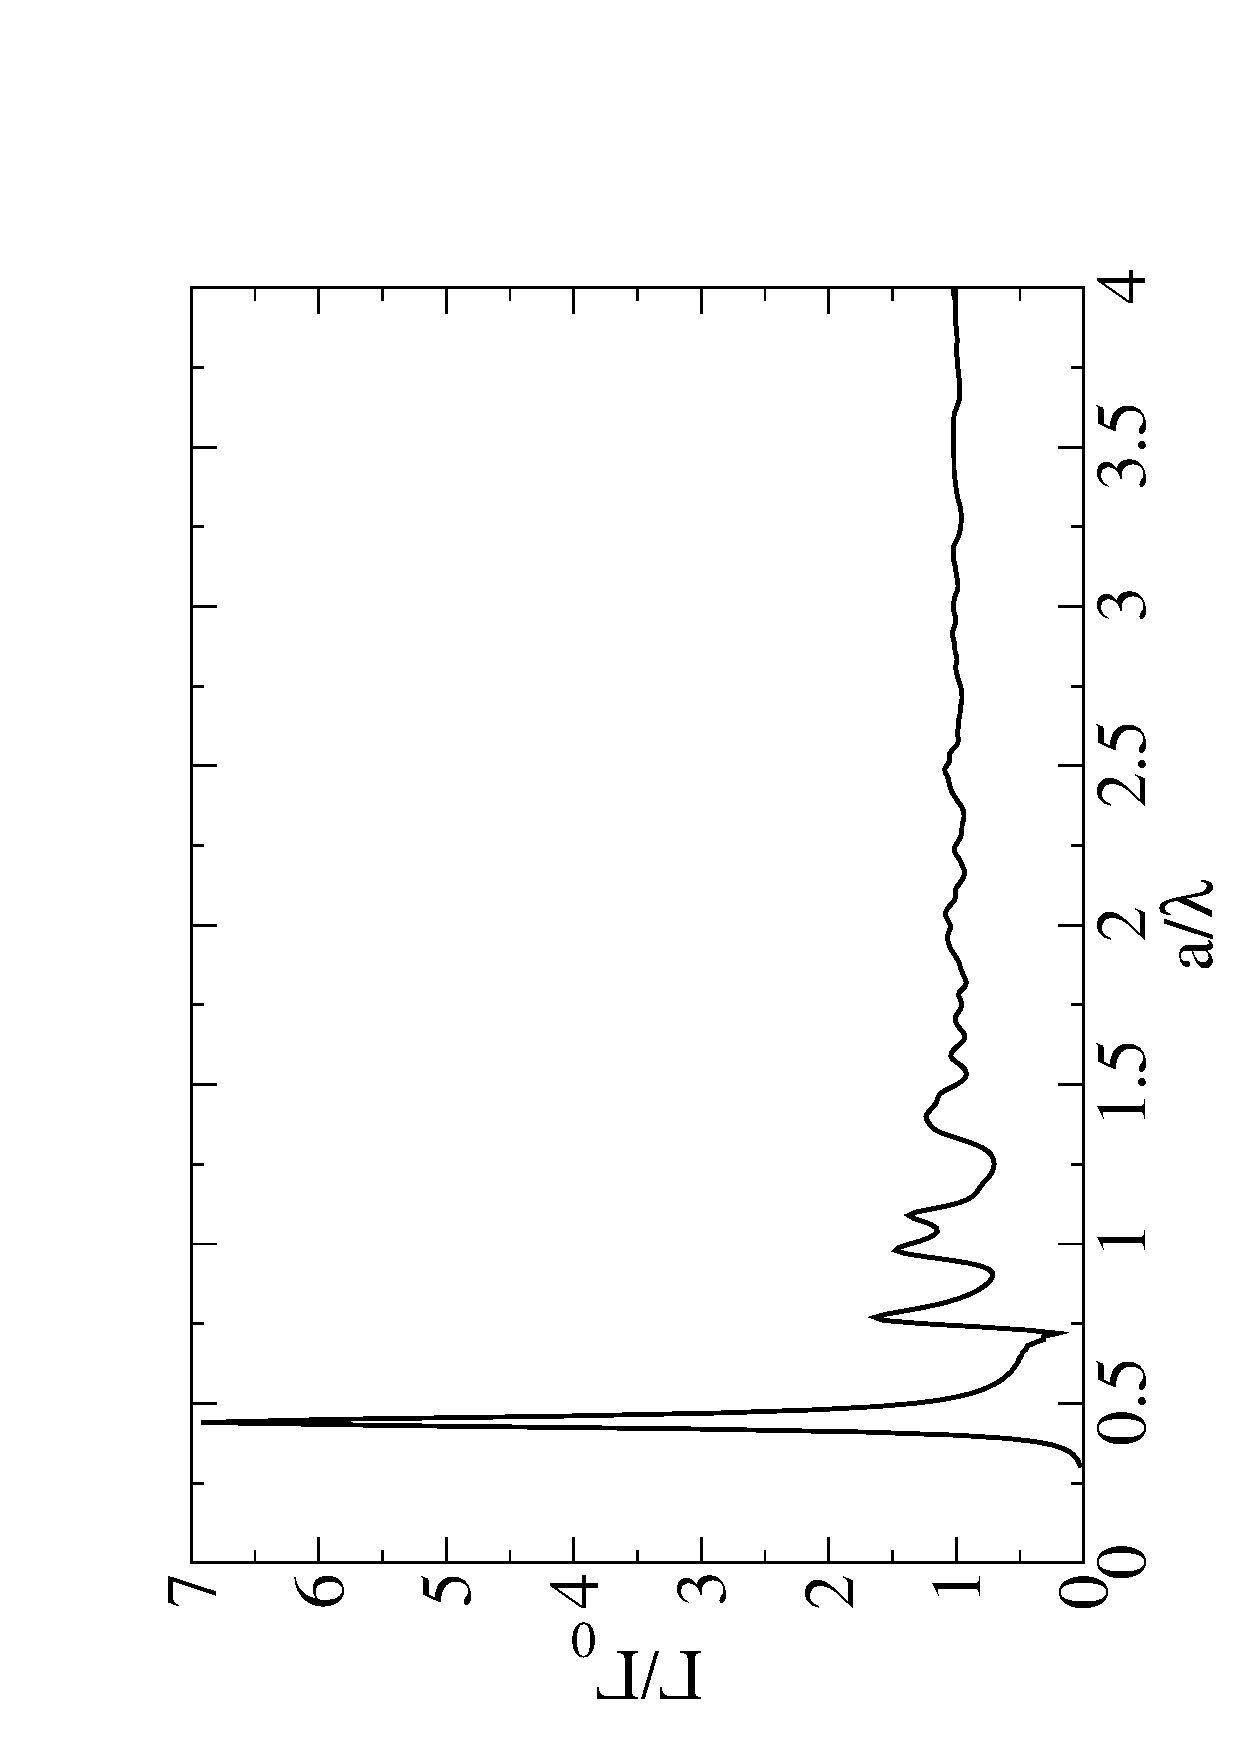
\includegraphics[angle=-90, width=9cm]{chapter_6/figures/fig_2} 
\par\end{centering}
\caption{Normalized decay rate of a crystalline structure for a system with
edge of $23$ particles (total system with $528$ particles). The maximum
can be found at $\frac{a}{\lambda}=0.44$.\label{fig:crystalline_spectrum}}
\end{figure}

Next, we fix the lattice parameter to $a=0.44\lambda$ and we analyse the decay rate distribution for disordered systems generated at different ordering temperatures ranging from $\theta \gg T_{c}$ ($\xi \rightarrow 0$) corresponding to a short-range correlated disorder to $\theta=T_{c}$ ($\xi \rightarrow \infty$), corresponding with a long-range correlated distribution of the vacancies. Results, for $10^{6}$ different configurations, are shown in Fig. (\ref{fig:temperature}).

\begin{figure}[h]
\begin{centering}
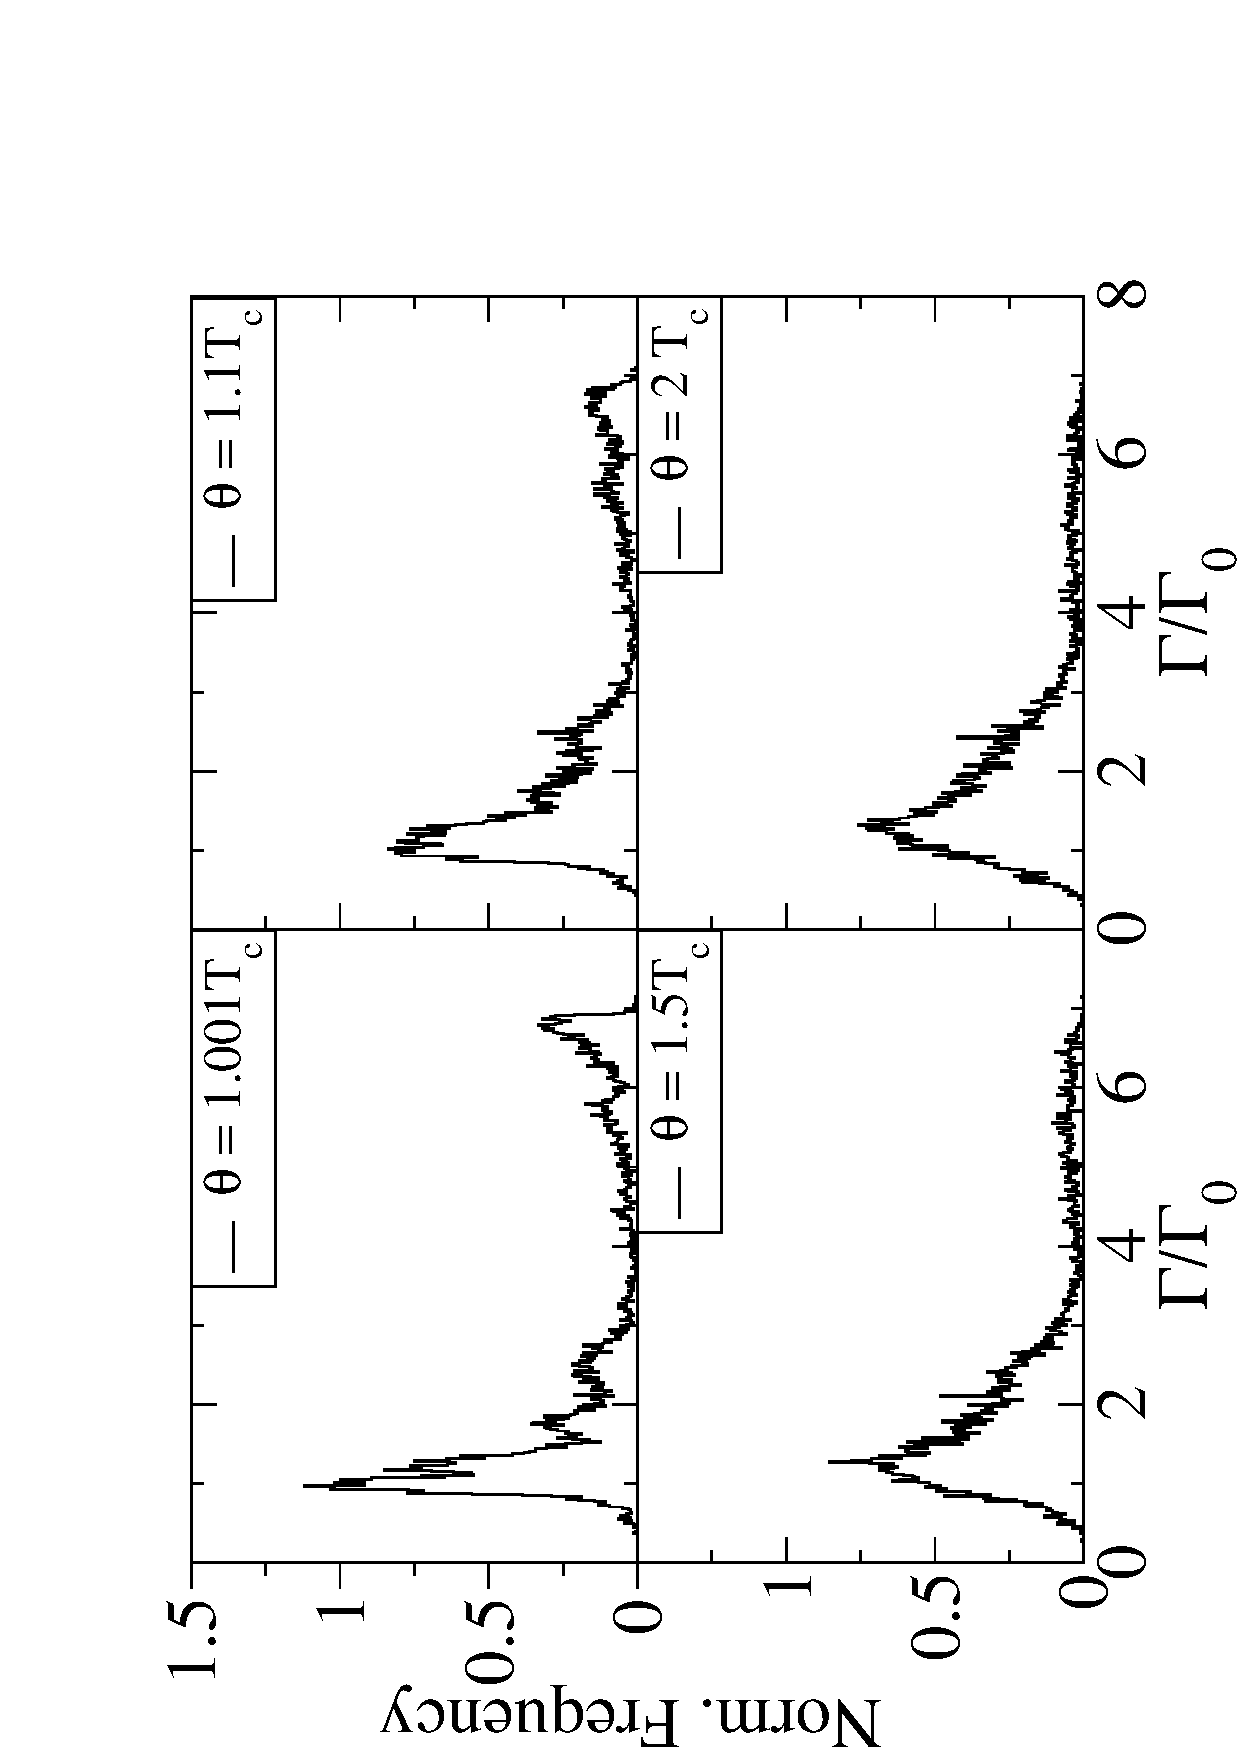
\includegraphics[angle=-90, width=11cm]{chapter_6/figures/fig_3} 
\par\end{centering}
\caption{Normalized histogram of the decay rate for $10^{6}$ different configurations
for a system with $D=23$.
\label{fig:temperature}}
\end{figure}

When the ordering temperature is large ($\theta \sim 2T_{c}$), we obtain a long-tailed distribution centered at $\Gamma/\Gamma_{0} \sim 1.3$, where some rare events are detected for values as high as  $\Gamma/\Gamma_{0} \sim 7$. Similar results have been previously reported \cite{Sapienza_2011, Froufe_2008}. However, as the ordering temperature decreases towards $T_{c}$, the correlation function between vacancies changes from an exponential decay to a power law  and the decay rate distribution reshapes dramatically. For $\theta=1.001T_{c}$, there is  no longer any long-tailed behaviour, but a bimodal distribution where the previously reported rare events increase considerably to build a new maximum centred at $\Gamma/\Gamma_{0} \sim 7$.\\
We have also analysed the possible presence of finite size effects by considering different lateral sizes ranging from $D=13$ to $D=63$ for $\theta=T_{c}$. Results are shown in Fig. (\ref{fig:histogram_all}). Note how all secondary maxima between $\Gamma/\Gamma_{0} \sim 1$ and $\Gamma/\Gamma_{0} \sim 7$ tend to smear out, while maxima at $\Gamma/\Gamma_{0} \sim 1$ and $\Gamma/\Gamma_{0} \sim 7$ are reinforced when the lateral size increases. 

\begin{figure}[h]
\begin{centering}
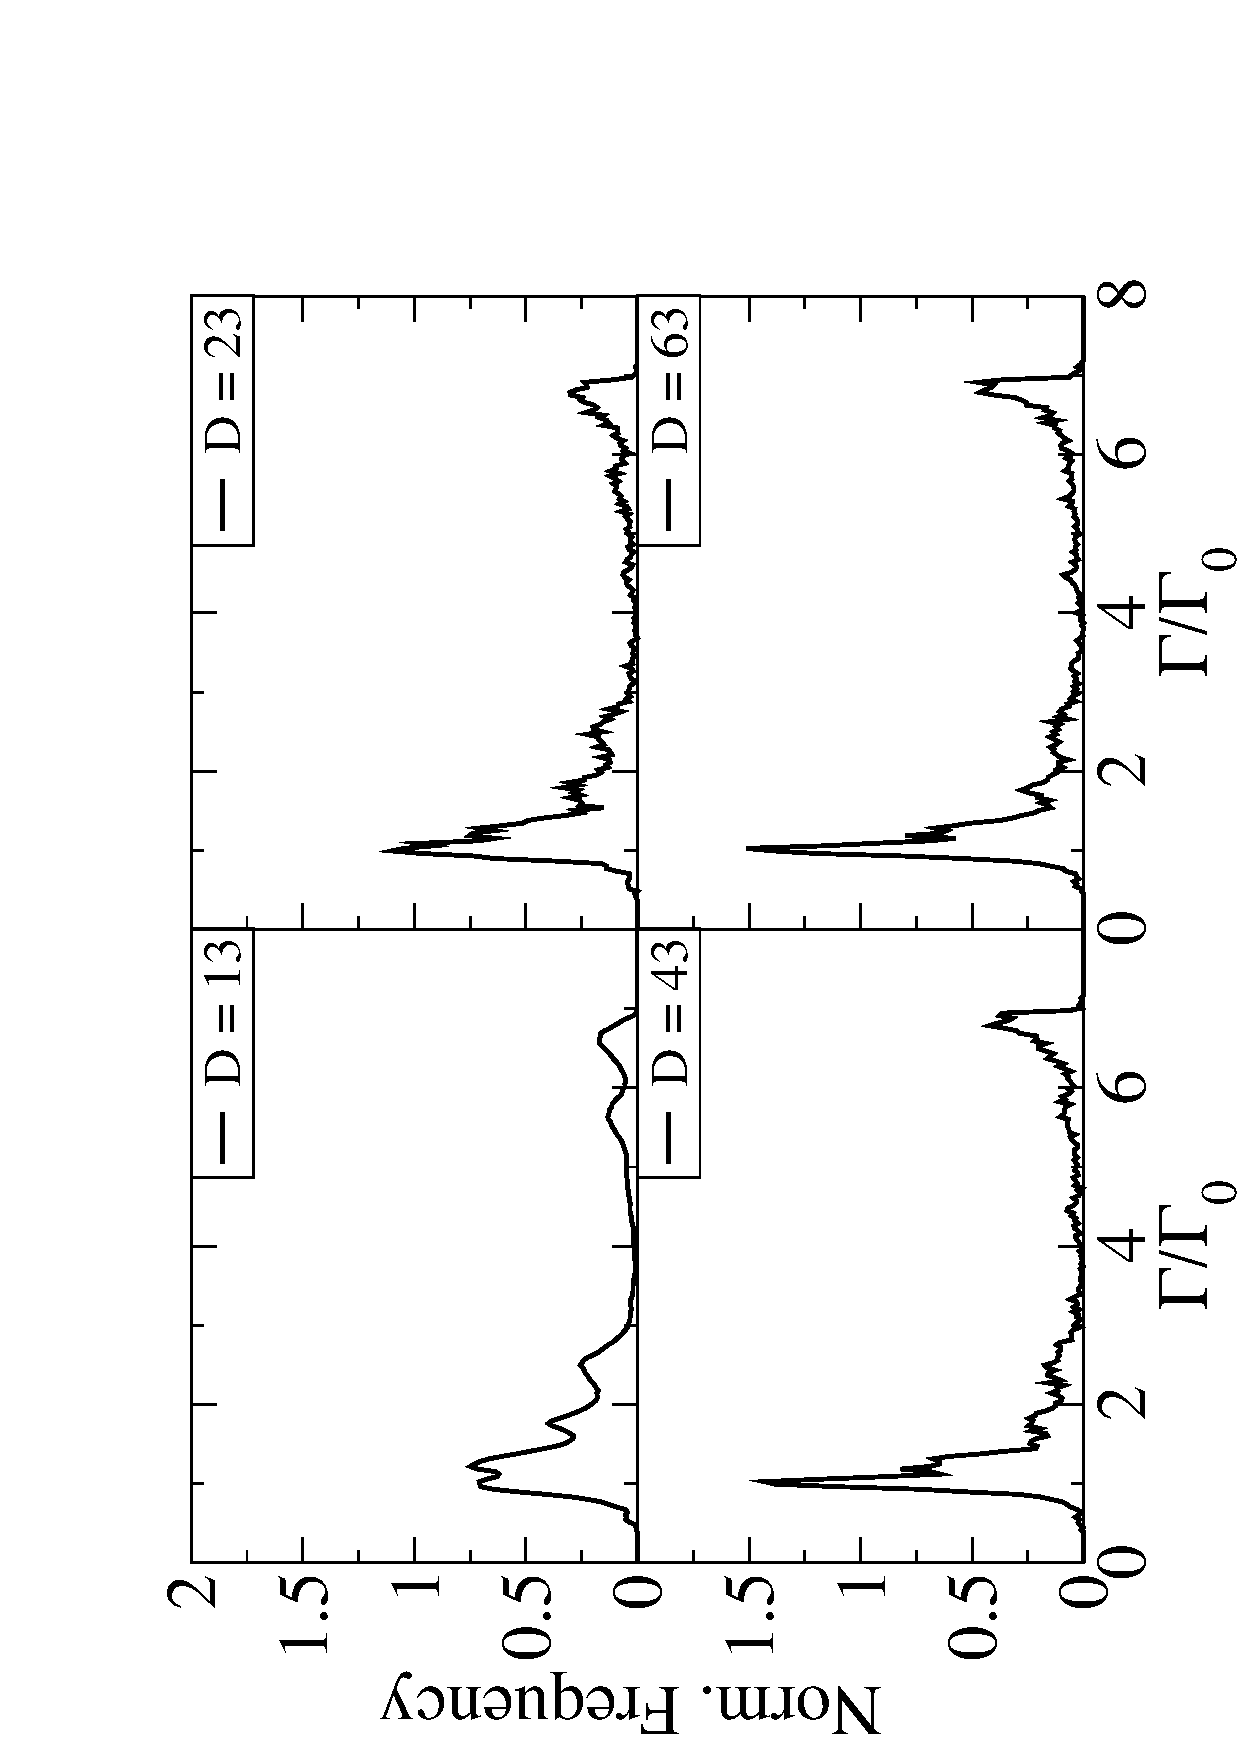
\includegraphics[angle=-90, width=11cm]{chapter_6/figures/fig_4} 
\par\end{centering}
\caption{Normalized histogram of the decay rate for $10^{6}$ different configurations at $\theta = T_{c}$.
The systems under study have an edge of $13$, $23$, $43$ and $63$, with a total of $168$, $528$, $1848$ and $3968$ particles repectively.\label{fig:histogram_all}}
\end{figure}

Large Purcell factors are due to optical modes confined around the source and are sustained by near-field interactions \cite{Sapienza_2011}. So systems with strong correlations, like the ones reported here, should promote an increase in the number of configurations where the emitting dipole is surrounded by clusters of dipoles allowing for field confinement. Due to the correlations, the two most probable configurations around the source are all sites occupied or unoccupied. To further analyse this idea, we plotted the histograms for systems with edge $23$, $43$ and $63$, for different values of the decay rate. The histograms represent the frequency of occupation for each position, normalized to the number of configurations. Black regions represent low occupation, while yellow regions represent sites with large occupation.
% we plotted the histogram of the frequency of occupation for each position normalized to the number of configurations, for different values of the decay rate. 
We focused our attention on $\frac{\Gamma}{\Gamma_{0}}=1.31\pm0.02$, corresponding to the maximum of the distribution for $\theta=2T_{c}$ ,when vacancies in the system are not correlated, and $\frac{\Gamma}{\Gamma_{0}}=0.98\pm0.02, 6.88\pm0.02$ corresponding to the two main maxima of the distribution for $\theta=T_{c}$, when vacancies in the system are correlated. Results are shown in Fig. (\ref{fig:col_hist}).



\begin{figure*}
\begin{centering}
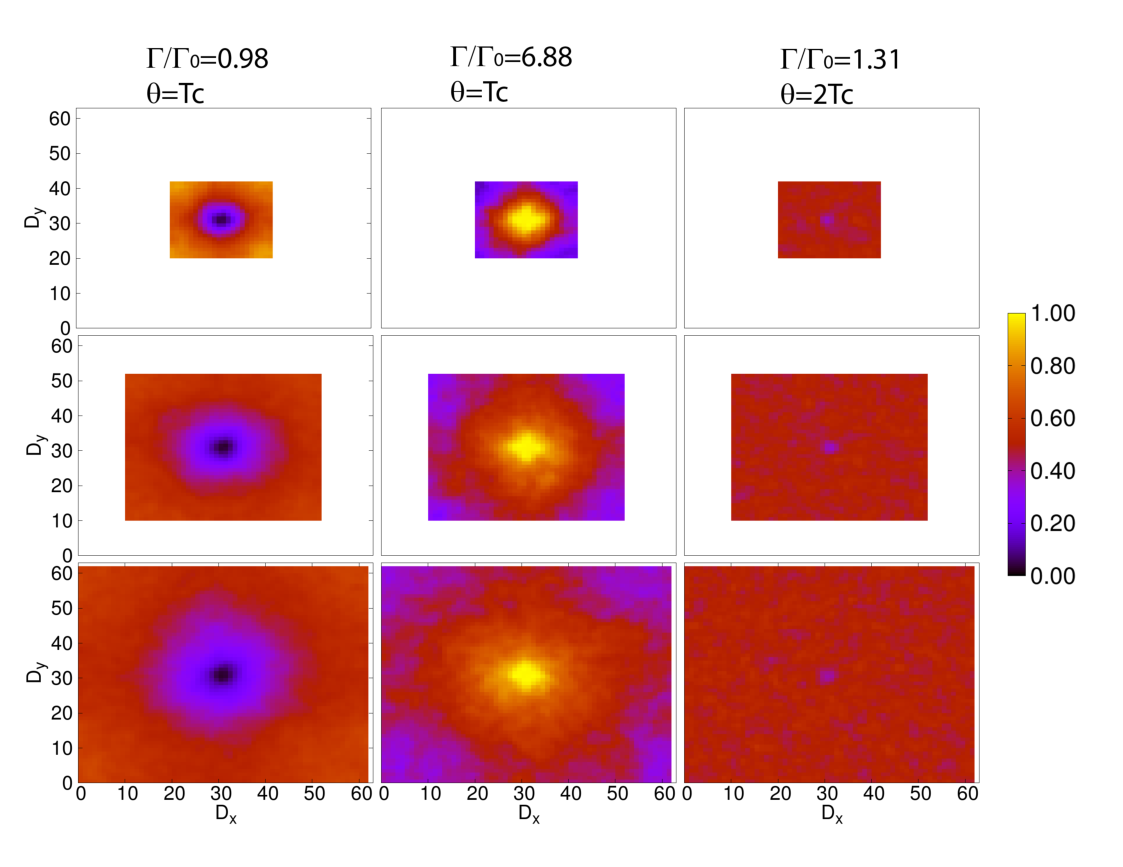
\includegraphics[width=0.8\paperwidth]{chapter_6/figures/fig_5} 
\par\end{centering}

\caption{Colormap histogram of the occupied positions for different size systems
(on vertical: $D=23$, $D=43$, $D=63$). We present three ordering temperatures, two at critical temperature ($T_{c}$), where the system present long range correlations, and one at high temperature ($2T_{c}$), where particles in the system are noncorrelated. Each histogram is normalized by the number of structures corresponding to each decay rate. \label{fig:col_hist}}
\end{figure*}




For $\frac{\Gamma}{\Gamma_{0}}=1.31$ we detect no special patterns, and dipoles are distributed almost randomly. However, for $\frac{\Gamma}{\Gamma_{0}}=6.88$ (corresponding to the second maximum for $\theta=T_{c}$) the dipoles distribution changes markedly. In this case, the emitting particle is clearly surrounded by scattering dipoles, allowing for confinement of the optical modes. This is in agreement with the attribution proposed by Sapienza \textit{et al.} \cite{Sapienza_2011} and clearly shows how large Purcell factors are boosted by long-range correlations in the disordered sample.  Interestingly, for the other maximum located at $\frac{\Gamma}{\Gamma_{0}}=0.98$, the situation is just the opposite and the emitting dipole is, on average, surrounded by vacancies where no field confinement is possible, entailing a dipole response similar to the one found in vacuum. This last effect is also fostered by the existence of long-range correlations when $\theta=T_{c}$. \\
In order to understand these effects, it is important to take into account that, at criticality, clusters of all sizes, containing either dipoles or vacancies,  exist on the system and the response due to larger clusters resembles the one found for the crystalline structure $\frac{\Gamma}{\Gamma_{0}} \sim 7$. However, when a noncorrelated distribution of vacancies is considered, the correlation length and the cluster's sizes are very small, and the detection of events with a large Purcell factor turns out to be very unlikely. The surface structure of the clusters in the Ising model for long-range correlation, \textit{i.e.} at criticality, is known to be fractal and scale invariant \cite{coniglio1989fractal}, like the clusters obtained for high filling factors in semicontinuous metal films experiments \cite{krachmalnicoff2010fluctuations}. These structures are responsible for surface plasmon localisation leading to a large increase in the decay rates. 

\section{Conclusion \label{chap:chap6_conclusions}}

In conclusion, the normalized fluorescent decay rate distribution has been analysed in a thermally disordered two-dimensional diluted dipole lattice where the correlation between vacancies may be tuned at will. When the ordering temperature is far from criticality, the correlation length is small, and the decay rate distribution shows the typical long-tailed shape where events with large Purcell factors are extremely rare. However, when the ordering temperature is close to criticality, the correlation length tends to infinity, turning the decay rate function into a bimodal distribution where large Purcell factor events are much more probable.\\
Thus, we have demonstrated the dramatic effect of correlations on the emission dynamics statistics. We have shown that, at constant density, the decay rate statistics can vary from mono-modal to bimodal distributions as the correlations increase.
%Our analysis shows that when vacancies are distributed with long-range correlations, enclose clusters of dipoles of all sizes, allowing for the existence of many configurations with optical modes confined around the source. 
 It is worth mentioning the analogy between our model system and related models in the field of optical lattices filled with cold atoms \cite{bloch2008many, bloch2012quantum, froufe2009threshold}, in particular for sparsely filled lattices. This analogy could open another way to study spatial correlations effects on the statistics of fluorescence lifetime.
